%%%%%%%%%%%%%%%%%%%%%%%%%%%%%%%%%%%%%%%%%%%%%%%%%%%%%%%%%%%%%%%%%%%%%%%%%%%
% Chapter: Cyber-Physical Systems
% Examples: examples/cps (Modelica models, the same equations in Python)
%%%%%%%%%%%%%%%%%%%%%%%%%%%%%%%%%%%%%%%%%%%%%%%%%%%%%%%%%%%%%%%%%%%%%%%%%%%

%%%%%%%%%%%%%%%%%%%%%%%%%%%%%%%%%%%%%%%%%%%%%%%%%%%%%%%%%%%%%%%%%%%%%%%%%%%
\section{Overview}
%%%%%%%%%%%%%%%%%%%%%%%%%%%%%%%%%%%%%%%%%%%%%%%%%%%%%%%%%%%%%%%%%%%%%%%%%%%
\nsl{An embedded system never works alone. It measures and influences a
physical process: the temperature of a room, the speed of a motor, the
position of a robot arm. Cyber-physical systems (CPS) are systems in which
this coupling of computation and physics is essential. They are often
distributed and connected, as in a car, a factory, a power grid or an
aircraft. Their behaviour can only be understood if both parts are
described together: the physics with differential equations, the software
with algorithms and state machines.
\newline
Because building and testing the real system is expensive and sometimes
dangerous, CPS are developed with models and simulation. This chapter
introduces the idea of CPS and the steps from a model to the real system.
It then shows how physical systems are modelled with the equation-based
language Modelica, using the free tool OpenModelica, and with a few lines of
Python.
\newpage}

\begin{description}
\item[{\rot\bf What is a cyber-physical system?}]~\\
\defn{def:Cyber-Physical System}
{\textbf{Cyber-physical systems} are integrations of computation with physical processes. Embedded computers and networks monitor and control the physical processes, usually with feedback loops where physical processes affect computations and vice versa. [Edward A.\ Lee, 2008]}
\bi
	\ite combination of mechanical, electrical, thermal, \ldots{} components with software and communication
	\ite examples: driver assistance systems, industrial robots, smart grids, medical devices, building automation
	\ite related terms: \textbf{Internet of Things} (focus on connectivity), \textbf{Industry 4.0} (production), \textbf{digital twin} (a model of a real system that is kept up to date with data from the system)
\ei
\os{\newpage}

\item[{\rot\bf The feedback loop}]~\\[-\lblskip]
\begin{figure}[!hbtp]
\begin{center}
\resizebox{0.85\textwidth}{!}{%
\begin{tikzpicture}[font=\sffamily\small,>=Stealth,
	b/.style={draw,thick,rounded corners,minimum width=30mm,minimum height=12mm,align=center}]
	\node[b,fill=green!15] (proc) at (0,0) {physical process\\(e.g.\ room, motor)};
	\node[b,fill=rwuviolet!15] (sens) at (-4.5,2.2) {sensors\\+ ADC};
	\node[b,fill=rwucyan!10] (comp) at (0,4.4) {computation\\(controller, state machine)};
	\node[b,fill=rwuviolet!15] (act) at (4.5,2.2) {actuators\\+ PWM, DAC};
	\node[b,fill=gray!10] (net) at (6.5,5.6) {network\\other systems};
	\draw[->,thick] (proc) -| node[pos=0.75,left,font=\sffamily\scriptsize]{measured values} (sens);
	\draw[->,thick] (sens) |- (comp);
	\draw[->,thick] (comp) -| (act);
	\draw[->,thick] (act) |- node[pos=0.25,right,font=\sffamily\scriptsize]{forces, heat, \ldots} (proc);
	\draw[<->,thick,dashed] (comp.north east) -- (net);
	\node[font=\sffamily\scriptsize] at (-4.5,4.9) {cyber};
	\node[font=\sffamily\scriptsize] at (-4.5,-0.6) {physical};
	\draw[dashed,gray] (-6.5,1.2) -- (7.5,1.2);
\end{tikzpicture}}
\caption{A cyber-physical system: computation and physical process in a closed loop}
\end{center}
\end{figure}
\bi
	\ite the physical process runs continuously in time; the computer samples and acts at discrete times
	\ite timing is part of the correctness: a controller that reacts too late can make the loop unstable
\ei
\os{\newpage}

\item[{\rot\bf From model to product}]~\\[-\lblskip]
\bi
	\ite the system is developed and tested in steps, replacing models by real parts one after the other
\ei
\begin{figure}[!hbtp]
\begin{center}
\resizebox{0.8\textwidth}{!}{%
\begin{tikzpicture}[font=\sffamily\small,>=Stealth,
	b/.style={draw,thick,rounded corners,minimum height=16mm,text width=30mm,align=center}]
	\node[b,fill=rwucyan!8] (mil) at (0,0) {\textbf{MiL}\\model in the loop\\controller model + plant model};
	\node[b,fill=rwucyan!15] (sil) at (4,0) {\textbf{SiL}\\software in the loop\\real code on the PC + plant model};
	\node[b,fill=rwuviolet!15] (pil) at (8,0) {\textbf{PiL}\\processor in the loop\\code on the target processor};
	\node[b,fill=rwuviolet!25] (hil) at (12,0) {\textbf{HiL}\\hardware in the loop\\real ECU + simulated plant in real time};
	\foreach \a/\b in {mil/sil,sil/pil,pil/hil} \draw[->,thick] (\a) -- (\b);
\end{tikzpicture}}
\caption{Test levels from the model to the real hardware}
\end{center}
\end{figure}
\bi
	\ite \textbf{HiL}: the real control unit runs against a real-time plant simulator -- dangerous or rare situations can be tested safely and repeatably
	\ite our Wokwi simulations are a kind of PiL test: the real firmware on a simulated processor
	\ite \textbf{FMI} 3.0 (2022): standard to exchange models between tools as \textbf{FMU}s for co-simulation
\ei
\os{\newpage}

\item[{\rot\bf Simulation of physical systems}]~\\[-\lblskip]
\bi
	\ite physical systems are described by \textbf{differential equations}, often with algebraic constraints (differential-algebraic equations, DAE)
	\ite models with lumped parameters (masses, springs, resistors) -- ordinary differential equations
	\ite continuous-time physics combined with discrete-time controllers and events (hybrid systems)
	\ite tools
	\bi
		\ite \textbf{block oriented}: MATLAB/Simulink, Xcos (Scilab) -- signals flow in one direction from block to block
		\ite \textbf{equation based} (object oriented): Modelica with OpenModelica (free) or Dymola (commercial) -- components are described by their physical equations
		\ite general programming languages: Python with \texttt{numpy}/\texttt{scipy}, Julia (ModelingToolkit)
	\ei
\ei
\os{\newpage}

\item[{\rot\bf Block oriented modelling}]~\\[-\lblskip]
\bi
	\ite the system is a diagram of blocks with inputs and outputs: gain, sum, integrator, transfer function
	\ite every connection has a fixed direction (causality): the modeller decides what is computed from what
\ei
\begin{figure}[!hbtp]
\begin{center}
\resizebox{0.6\textwidth}{!}{%
\begin{tikzpicture}[font=\sffamily\small,>=Stealth,
	b/.style={draw,thick,minimum width=14mm,minimum height=10mm}]
	\node[b] (gain) at (0,0) {$-a$};
	\node[b] (int) at (3,0) {$\displaystyle\int dt$};
	\draw[->,thick] (gain) -- node[above]{$\dot x$} (int);
	\draw[->,thick] (int) -- (5,0) node[right]{$x$};
	\draw[->,thick] (4.3,0) |- (1.5,-1.4) -| ($(gain.west)+(-0.6,0)$) -- (gain.west);
	\fill (4.3,0) circle (1.5pt);
	\node[below,font=\sffamily\scriptsize] at (3,0.9) {$x(0)=1$};
\end{tikzpicture}}
\caption{Block diagram of $\dot x = -a\,x$: the output of the integrator is fed back}
\end{center}
\end{figure}
\bi
	\ite natural for control engineering and signal processing
	\ite for physical networks (electrical circuits, mechanics) the modeller must first solve the equations for the right variables by hand -- this is what equation-based tools avoid
\ei
\os{\newpage}
\end{description}

%%%%%%%%%%%%%%%%%%%%%%%%%%%%%%%%%%%%%%%%%%%%%%%%%%%%%%%%%%%%%%%%%%%%%%%%%%%
\section{Modelling with Modelica}
%%%%%%%%%%%%%%%%%%%%%%%%%%%%%%%%%%%%%%%%%%%%%%%%%%%%%%%%%%%%%%%%%%%%%%%%%%%
\nsl{Modelica is a language for describing physical systems by equations. A
model states which relations hold, for example Ohm's law $u = R \cdot i$,
without saying which variable is computed from which. The compiler sorts the
equations, solves them symbolically where possible and generates simulation
code. Components can be connected like real parts: connecting a resistor to
a capacitor automatically produces Kirchhoff's laws. Modelica is
standardised by the Modelica Association. OpenModelica is a free
implementation with a graphical editor (OMEdit) and an extensive standard
library for electrical, mechanical, thermal, fluid and control components.}

\begin{description}
\item[{\rot\bf Features of Modelica / OpenModelica}]~\\[-\lblskip]
\bi
	\ite \textbf{equation based} (acausal): equations instead of assignments -- the tool decides the order of computation
	\ite \textbf{object oriented}: classes, instances, inheritance, packages; parameters separate from the structure (a resistor model, used with different values)
	\ite \textbf{multi-domain}: electrical, mechanical, thermal, hydraulic, \ldots{} components in one model
	\ite \textbf{connectors} with potential variables (voltage, temperature) and flow variables (current, heat flow): \texttt{connect()} creates the equations ``potentials equal, sum of flows zero''
	\ite physical units for all quantities (\texttt{unit = "V"}) -- the tool checks them
	\ite graphical (drag and drop in OMEdit) and textual modelling of the same model
	\ite export as FMU for co-simulation; code generation for controllers
\ei
\os{\newpage}

\item[{\rot\bf OpenModelica: graphical modelling}]~\\[-\lblskip]
\begin{figure}[!hbtp]%
     \begin{center}
	  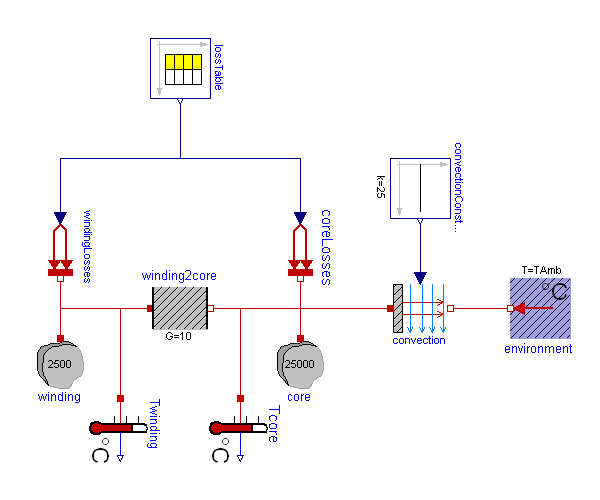
\epsfig{file=figures/Fig_3_3_OpenModelica,width=0.8\textwidth}\\
	  \caption{OpenModelica model of a heat transfer}
     \end{center}
\end{figure}
\os{\newpage}

\item[{\rot\bf First elements of Modelica}]~\\[-\lblskip]
\bi
	\ite data types: \texttt{Real} (64 bit floating point), \texttt{Integer}, \texttt{Boolean}, \texttt{String}, enumerations
	\ite \texttt{parameter}: constant during a simulation, can be changed between simulations
	\ite \texttt{der(x)}: time derivative $\dot x$
	\ite \texttt{start}: initial value; \texttt{fixed = true}: the initial value must hold exactly
	\ite example: $\dot x = -a \cdot x$
\ei
\begin{lstlisting}[language={}]
model HDE
  Real x(start = 1, fixed = true);
  parameter Real a = 1;
equation
  der(x) = -a*x;
end HDE;
\end{lstlisting}
\os{\newpage}

\begin{figure}[!hbtp]
     \begin{center}
	  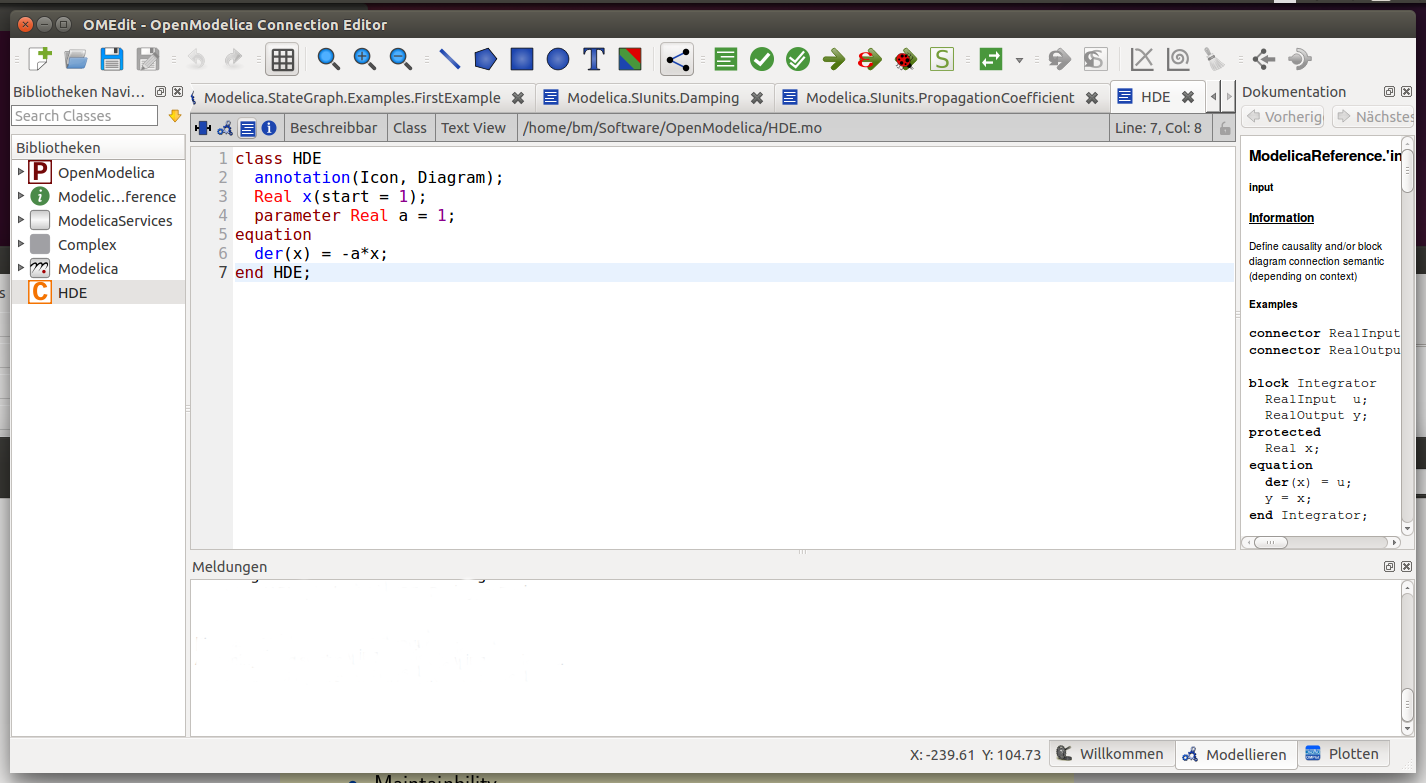
\epsfig{file=figures/Fig_3_4_HDE_OMEdit,width=0.75\textwidth}\\
	  \caption{Model HDE in OMEdit}
     \end{center}
\end{figure}
\os{\newpage}

\begin{figure}[!hbtp]
     \begin{center}
	  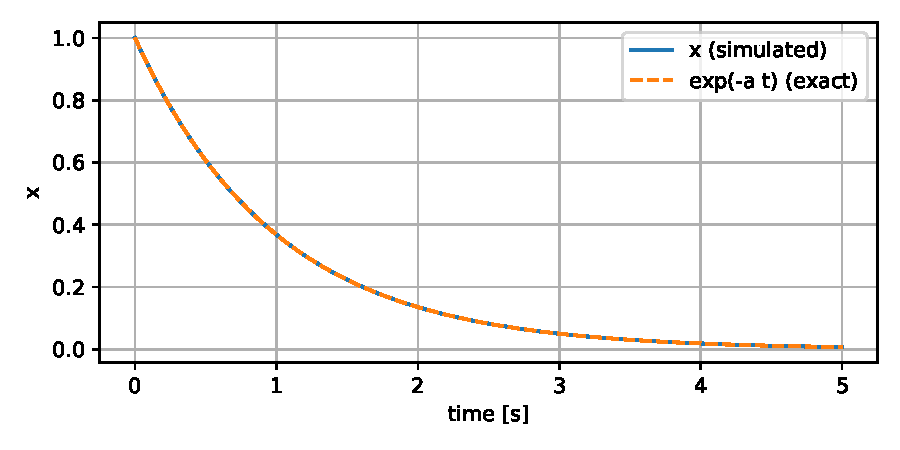
\epsfig{file=figures/cps_hde.pdf,width=0.75\textwidth}\\
	  \caption{Solution of the model HDE: simulation and exact solution $x(t) = e^{-a t}$}
     \end{center}
\end{figure}
\os{\newpage}

\item[{\rot\bf Differential-algebraic equations: the pendulum}]~\\[-\lblskip]
\bi
	\ite a model can contain algebraic equations (without derivatives) besides the differential equations
	\ite example: a planar pendulum, a mass $m$ on a rod of length $L$; the rod force $F$ is unknown
\ei
\begin{minipage}{0.3\textwidth}
\begin{center}
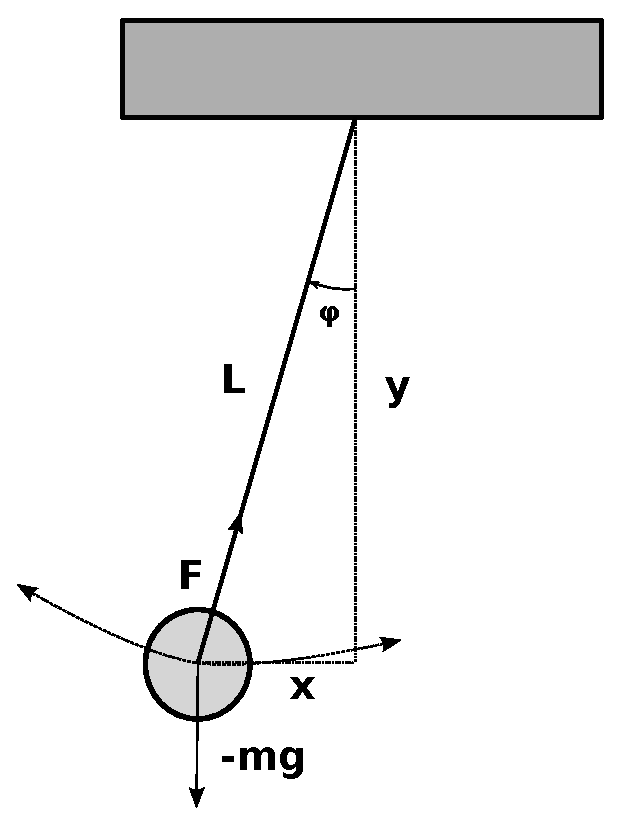
\epsfig{file=figures/Fig_3_6_Pendulum,width=0.8\textwidth}
\end{center}
\end{minipage}
\begin{minipage}{0.65\textwidth}
\begin{eqnarray*}
m\,\dot{v}_x &=& -\frac{x}{L}\,F \\
m\,\dot{v}_y &=& -\frac{y}{L}\,F - m\,g \\
\dot{x} &=& v_x \\
\dot{y} &=& v_y \\
x^2 + y^2 &=& L^2
\end{eqnarray*}
\end{minipage}
\bi
	\ite 5 equations for 5 unknowns ($x, y, v_x, v_y, F$); the last equation is the constraint of the rod
\ei
\os{\newpage}

\item[{\rot\bf The pendulum in Modelica}]~\\[-\lstskip]
\begin{lstlisting}[language={}]
model Pendulum "Planar pendulum"
  parameter Real m = 1, g = 9.81, L = 0.5;
  Real F;
  Real x(start = 0.5, fixed = true), y(start = 0);
  Real vx, vy;
equation
  m*der(vx) = -(x/L)*F;
  m*der(vy) = -(y/L)*F - m*g;
  der(x) = vx;
  der(y) = vy;
  x^2 + y^2 = L^2;   // algebraic equation (constraint of the rod)
end Pendulum;
\end{lstlisting}
\bi
	\ite the equations are written as in the physics book; OpenModelica reduces the DAE (index reduction) and chooses the state variables itself
\ei
\os{\newpage}

\begin{figure}[!hbtp]
     \begin{center}
	  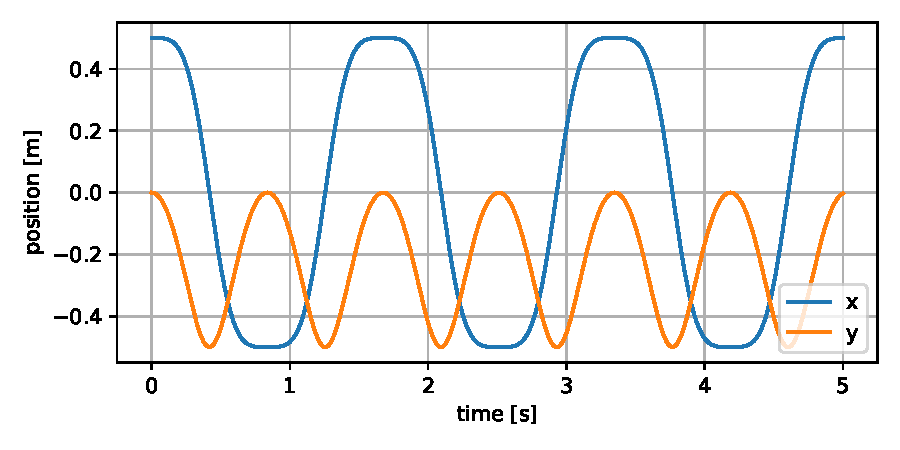
\epsfig{file=figures/cps_pendulum.pdf,width=0.8\textwidth}\\
	  \caption{Horizontal and vertical position of the pendulum, started with the rod horizontal}
     \end{center}
\end{figure}
\bi
	\ite $y$ is always $\le 0$: the mass swings below the pivot; the period is longer than for small angles
\ei
\os{\newpage}

\item[{\rot\bf Classes and instances}]~\\[-\lblskip]
\bi
	\ite every object has a class that defines its data and its behaviour
	\ite a class has variables (constants, parameters, computed values), equations, and can contain instances of other classes
\ei
\begin{lstlisting}[language={}]
class Point "Point in a three-dimensional space"
  Real x;
  Real y;
  Real z;
end Point;

class Triangle
  Point point1;
  Point point2;
  Point point3;
end Triangle;

class Triangle2 "with modification of an instance"
  Point point1(x = 1, y = 2, z = 3);
  Point point2;
  Point point3;
end Triangle2;
\end{lstlisting}
\os{\newpage}

\item[{\rot\bf An electrical example}]~\\[-\lblskip]
\begin{minipage}{0.35\textwidth}
\begin{center}
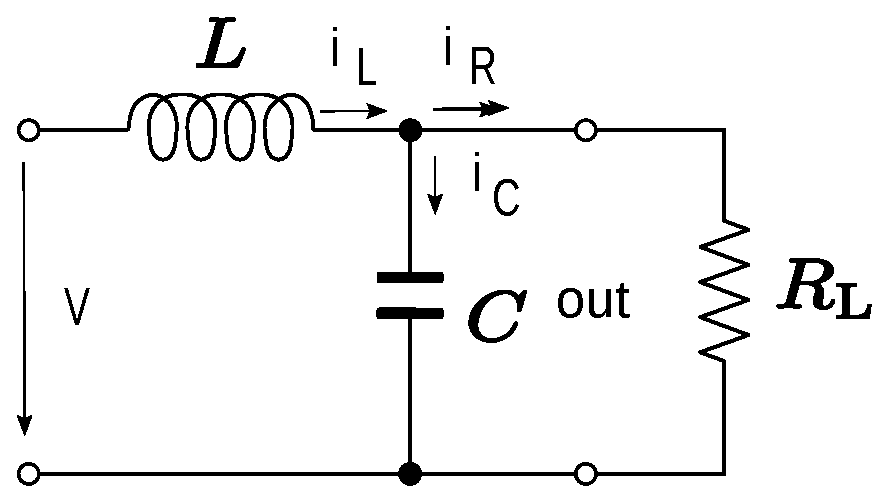
\epsfig{file=figures/Fig_3_8_RLC,width=0.9\textwidth}
\end{center}
\end{minipage}
\begin{minipage}{0.6\textwidth}
\begin{lstlisting}[language={}]
model RLC1 "A resistor-inductor-capacitor circuit"
  type Voltage = Real(unit = "V");
  type Current = Real(unit = "A");
  parameter Voltage Vb = 24 "Battery voltage";
  parameter Real L(unit = "H") = 1;
  parameter Real R(unit = "Ohm") = 100;
  parameter Real C(unit = "F") = 1e-3;
  Voltage V;
  Current i_L, i_R, i_C;
equation
  V = i_R*R;
  C*der(V) = i_C;
  L*der(i_L) = Vb - V;
  i_L = i_R + i_C;
end RLC1;
\end{lstlisting}
\end{minipage}
\os{\newpage}

\begin{figure}[!hbtp]
     \begin{center}
	  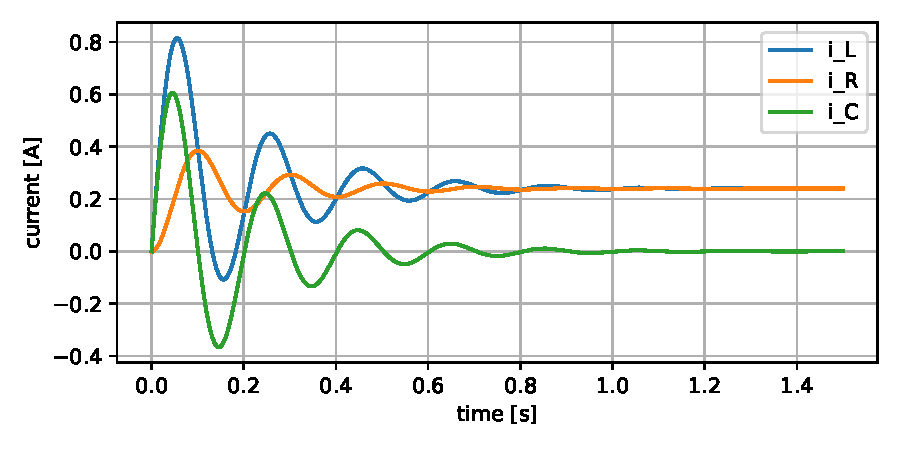
\epsfig{file=figures/cps_rlc.pdf,width=0.8\textwidth}\\
	  \caption{Currents in the RLC circuit after switching on the battery}
     \end{center}
\end{figure}
\bi
	\ite damped oscillation ($\omega_0 = 1/\sqrt{LC} \approx 31.6$\,s$^{-1}$, i.e.\ about 5\,Hz); final state $i_L = i_R = V_b/R = 0.24$\,A, $i_C = 0$
\ei
\os{\newpage}

\item[{\rot\bf The same equations in Python}]~\\[-\lstskip]
\begin{lstlisting}[language=Python]
from scipy.integrate import solve_ivp

Vb, L, R, C = 24.0, 1.0, 100.0, 1e-3

def rlc(t, s):            # state: capacitor voltage V, inductor current i_L
    V, iL = s
    return [(iL - V / R) / C,      # C dV/dt   = i_C = i_L - V/R
            (Vb - V) / L]          # L di_L/dt = Vb - V

sol = solve_ivp(rlc, (0, 1.5), [0.0, 0.0], max_step=1e-3)
print("final i_L =", sol.y[1][-1])   # 0.240 A
\end{lstlisting}
\bi
	\ite here the equations had to be solved for the derivatives by hand -- for the RLC circuit easy, for the pendulum DAE not (we used the angle as the only state)
	\ite this is exactly the work Modelica does automatically for large models
	\ite the plots of this chapter were created with this script (\texttt{examples/cps/simulate.py}, runs on Replit)
\ei
\os{\newpage}

\item[{\rot\bf Exercises}]~\\[-\lblskip]
\bi
	\ite Simulate \texttt{HDE}, \texttt{Pendulum} and \texttt{RLC1} in OpenModelica and compare with the plots of the Python script.
	\ite Change $R$ in the RLC circuit to $10\,\Omega$ and $1000\,\Omega$. When does the circuit stop oscillating? Compare with the condition $R = \frac{1}{2}\sqrt{L/C}$.
	\ite Build the RLC circuit graphically from the Modelica standard library (\texttt{Modelica.Electrical.Analog}) and compare the generated equations with \texttt{RLC1}.
	\ite Add a two-point controller to a heated room model: heating on below 20\,$^\circ$C, off above 21\,$^\circ$C. How does the hysteresis influence the switching frequency?
\ei
\end{description}
